%%%%%%%%%%%%%%%%%%%%%%%%%%%%%% -*- Mode: Latex -*- %%%%%%%%%%%%%%%%%%%%%%%%%%%%
%% project.plan.tex -- 
%% Author          : Philip Johnson
%% Created On      : Fri Jan 13 19:47:12 2012
%% Last Modified By: Philip Johnson
%% Last Modified On: Tue Jan 24 13:42:43 2012
%%%%%%%%%%%%%%%%%%%%%%%%%%%%%%%%%%%%%%%%%%%%%%%%%%%%%%%%%%%%%%%%%%%%%%%%%%%%%%%

\subsection{Project plan}

\begin{figure}[th!]
  \begin{center}
   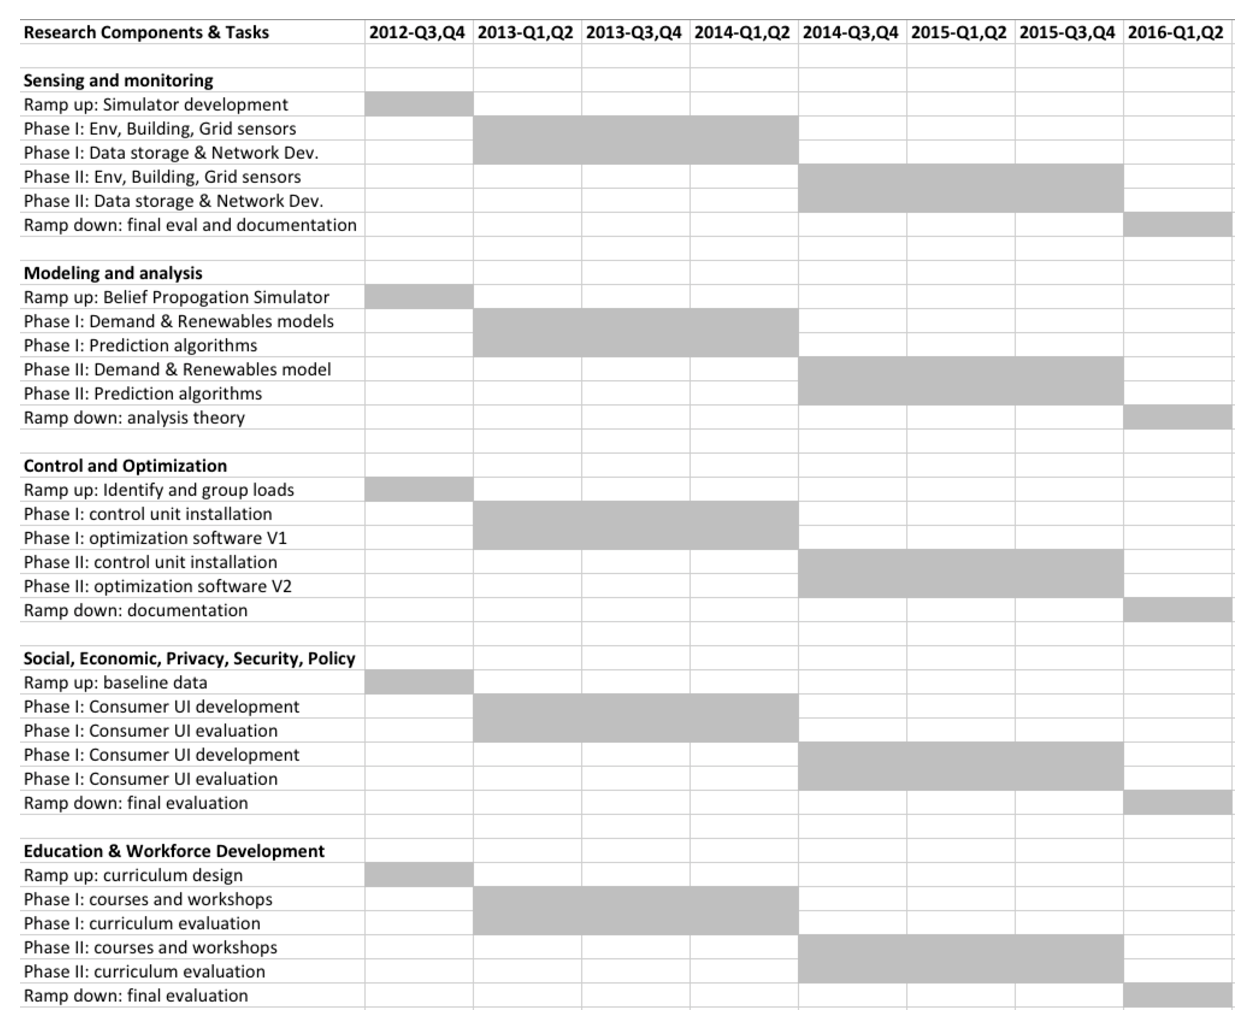
\includegraphics[width=0.9\textwidth]{fig/sep-timeline.eps}
   \caption{Work breakdown structure.}
  \label{fig:timeline}
  \end{center}
\end{figure}

Figure \ref{fig:timeline} illustrates the project timeline, organized by
the five research components.  The four years of this project are broken
down into four phases: a six month ``ramp up'' phase at the start of the
project, followed by two eighteen month phases in which we iteratively
develop and evaluate the microgrid, followed by a six month ``ramp down''
phase in which we focus on documentation, evaluation, and other activities
necessary to allow maximal external use of the knowledge and skills gained
during this project. 

The goal of the initial six month ramp up phase is to complete all of the
startup activities necessary to ensure a successful Phase I implementation
of the microgrid.  For all research components, this involves hiring of
personnel and initial meetings to review literature and become familiar
with relevant issues and technologies. For the sensing and monitoring
component, the ramp up period also involves the development of a simple
server based upon historical data that can provide simulated data about
building loads, environmental data, and grid state.  This simulated data
will be relatively imprecise given the short time available for
implementation, but its goal is to simply enable other research components
to make progress prior to complete installation of sensors.  The modeling
and analysis component will also create a simulator during the ramp up
phase, in this case for a belief propogation network appropriate to the
microgrid. The control and optimization component will research historical
loads and assess control unit types and applicability.   The social,
economic, privacy, security, and policy (SEPSP) research component will
obtain baseline data regarding energy use, attitudes, and concerns
among the university stakeholders. Finally, the education and workforce
development research component will work on curriculum during the ramp up
phase. 

After ramp up, the project begins two eighteen month cycles of microgrid
design, implementation, and evaluation.   We designed the project
so that by the end of year two of this four year project, we will have
created a functional microgrid, though not complete or optimal. 
By the end of Phase I, the sensors and monitoring research component will
have installed an initial set of environmental, grid, and building
sensors and this data will be provided for use in modeling, analysis,
control, and optimization.  Based upon Phase I experiences, the sensors and
monitoring research component will install additional sensors or modify
existing ones to improve the quality of grid performance in Phase II.

A similar iterative approach is employed in the other research
components. During Phase I, the modeling and analysis research component
will create models of both energy demand and renewable resource production
and build an initial prediction algorithm using the data provided by Phase
I sensors and monitoring.  The strengths and weaknesses of these initial
models and the data they are based upon will be evaluated at the end of
Phase I and used to construct more robust and performance models and
prediction algorithms in Phase II.  Similarly, the control and optimization
research component will implement initial control mechanisms during Phase
I, and the results will be used to generate Phase II requirements for the
modeling and analysis and sensors and monitoring research components.   

The SEPSP research component during Phase I and II is similarly iterative,
but here the focus is on creating and evaluating user interfaces that
result in active participation by campus members in the management of the
grid.  Finally, the education and workforce development components will
focus during Phase I on more general curriculum while the micro grid is
still under initial construction.  During Phase II, the curriculum can be
refocused to incorporate ``live'' analysis of the running microgrid and its
operational state. 

The project plan provides for a six month ``ramp down'' period at the
conclusion of the four years.  The goal during this period is to ensure
that we  create curriculum, publications, software, hardware, and
documentation of maximal utility to others wishing to engage in microgrid
development either in Hawaii or on the mainland.   In addition, the final
six months serves as a ``buffer'' period in the event that Phase I or Phase
II takes longer than expected. 






